%!TEX root = uist14.tex
\section{Iteration 1: IR-based Head Orientation with List Refinement}

\subsection{Interaction Flow}
\bjoern{I pulled this from the earlier paper}

\begin{figure}[t!]
\centering
\includegraphics[width=\columnwidth]{figures/stepbystep_small.png}
\caption{Targeting interaction: when users turn towards a controllable appliance (A$\rightarrow$B), the appliance shows immediate visual feedback (red LED) (B). Users confirm that they wish to connect to this appliance with a tap (C) which triggers connection feedback (blue LED) on the appliance.}
\label{fig:interaction}
\vspace{0.1in}
\includegraphics[width=\columnwidth]{figures/stepbystep_multi_small.png}
\caption{When multiple appliances are within range, they all have red LEDs illuminated for feedback (A). When users initiate connections, all target appliances toggle on blue LEDs while the currently selected one blinks (B). Swiping on the touchpad traverses among responding appliances (C).}
\label{fig:interaction_multi}
\end{figure}

\begin{figure}[t]
\centering
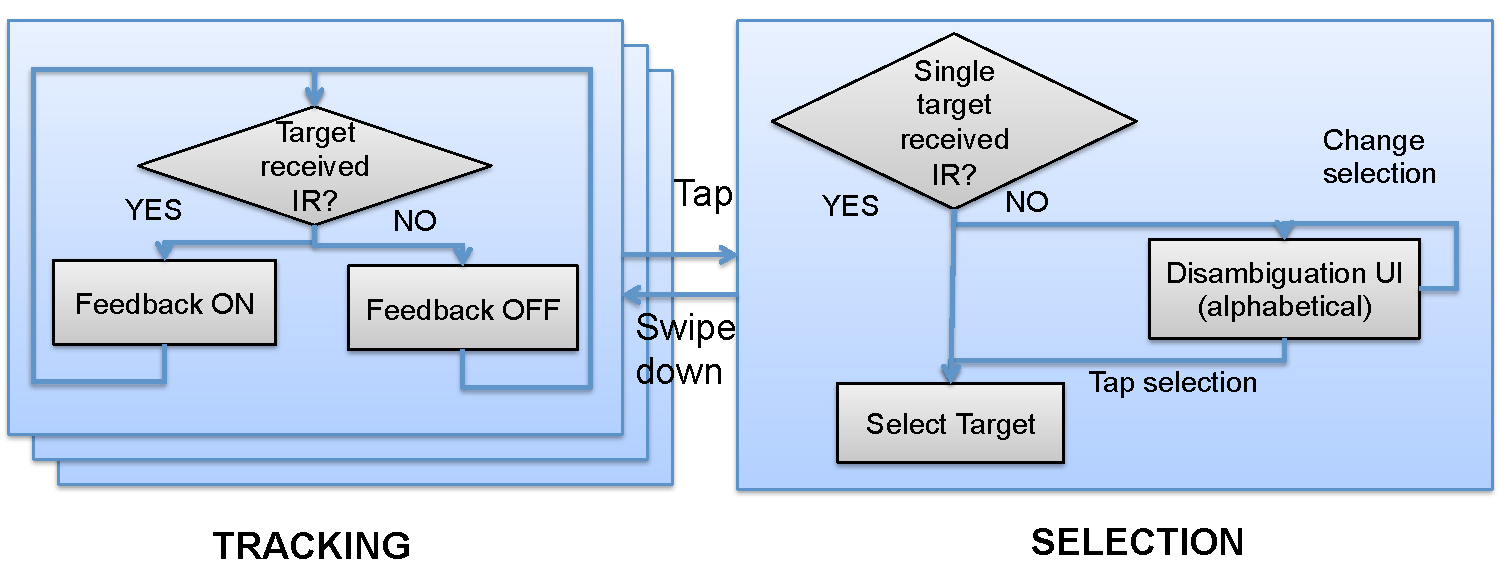
\includegraphics[width=1.0\columnwidth]{figures/selectflow01.pdf}
\caption{Head orientation selection flowchart for our first design.}
\label{fig:selectflow01}
\end{figure}

{\bf Look:} Users looking in the general direction of the intended target.
Glass periodically sends a device id through its IR emitter analogous to Patel's approach~\cite{patel_2-way_2003}. Target appliances have IR receivers and offer immediate visual feedback by toggling a red LED whenever a valid id is received (Figure~\ref{fig:interaction}B). This enables {\em scanning} the environment with one's gaze to see which appliances can be controlled.

{\bf Initiate:} Users confirm their desire to connect to an appliance by tapping on the Glass touchpad. After they are connected, the target appliance toggles on a blue LED as visual feedback (Figure~\ref{fig:interaction}C). The next section on disambiguation deals with cases in which multiple appliances received valid IR signals. At this point, all further communication switches over to the 802.15.4 wireless network so that line of sight to the target is no longer needed.

{\bf Refinement:}
Head orientation only indicates a general area of visual interest. It does not necessarily match gaze orientation as extra-ocular muscles can move the eyes. The IR beam of our device also has a certain spread . In an environment dense with potential targets, multiple targets could be within range. Users can tell when multiple feedback LEDs in the environment illuminate (Figure~\ref{fig:interaction_multi}A). To disambiguate, users can either move to adjust their head position, or, alternatively, call up a disambiguation dialog on the Glass display. The dialog presents a list filtered to only those appliances that are within IR range, while appliances also use blue LED as visual cues: all responding appliances light up LEDs while the currently selected one blinks (Figure~\ref{fig:interaction_multi}B). Users navigate the list using the touchpad (Figure~\ref{fig:interaction_multi}C), and then continue their interaction as described above.

\subsection{Implementation}
\begin{figure}[t]
\centering
\includegraphics[width=0.7\columnwidth]{figures/tube_from_top.jpg}
\caption{Our augmented Glass prototype has a frame-mounted infrared emitter.}
\label{fig:glass}
\end{figure}
\begin{figure}[t]
\centering
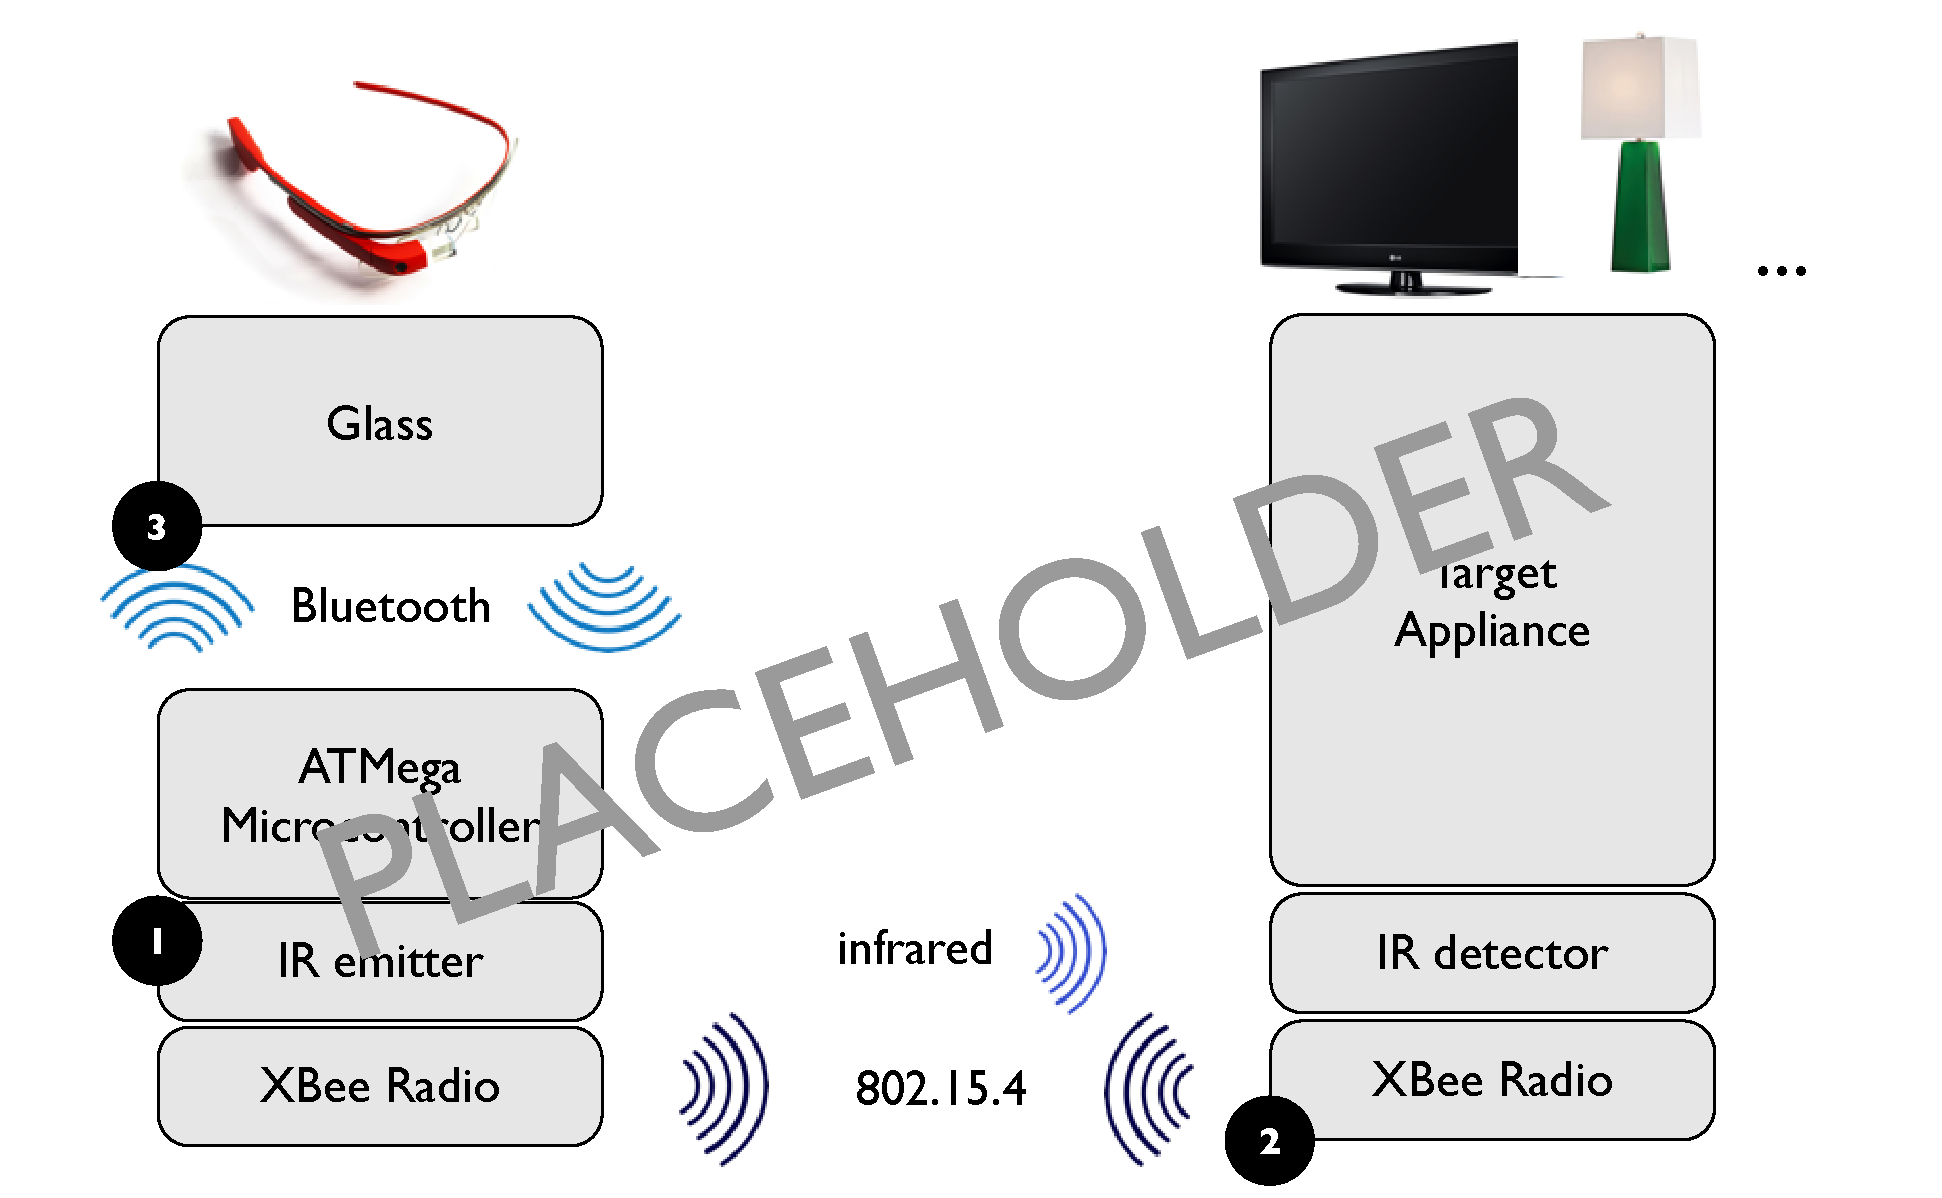
\includegraphics[width=1.0\columnwidth]{figures/architecture}
\caption{In our system architecture, selection is initiated through infrared but confirmed over 802.15.4. This permits wearers to move their head freely after connecting to an appliance. In the research prototype, users have to carry an additional microcontroller board that marshals messages between Glass' Bluetooth radio an IR/802.15.4, but our custom hardware could also be integrated into the wearable device.}
\label{fig:architecture}
\end{figure}

Our prototype consists of a Google Glass Explorer Edition device, augmented with an infrared emitter that is mounted on the frame, pointing out in the direction of the wearer's view (Figure~\ref{fig:glass}). The IR emitter LED is mounted in a \bjoern{3D printed housing which can be adjusted so the emitter can point straight forward for different head shapes}.

Our measurements suggest that IR communication can be targeted to an area about 60-120cm in diameter, up to 5m in front of the user. These values are a reasonable match for selecting targets in a room-size environment. A wider beam would lead to an increased chance of multiple appliances receiving IR signals simultaneously. A narrower beam will make targeting more challenging, given the precision constraints of human head movement.

In our prototype, Glass communicates over Bluetooth to an additional microcontroller board the user has to wear (Atmel ATMega256). This board marshals XBee to Bluetooth messages in both directions and also controls the IR LED mounted on the Glass frame (Figure~\ref{fig:architecture}). This architecture was chosen for reasons of expediency and we do not claim optimality for our design decisions. Future head-mounted devices could clearly integrate IR emitters; the choice of local wireless technology could also change. In particular, one could substitute WiFi modules or design an all-Bluetooth network.


\subsection{Device Characterization}
We determined the usable range and accuracy empirically with one IR emitter and two IR receivers. The IR emitter constantly sent out an id signal. The receivers that correctly received the signal turn their LED on for 300 ms. Our measurements suggest that IR communication can be targeted to an area about 2--4' in diameter, up to 16' in front of the user. These values are a reasonable match for selecting appliances in a room-size environment. A wider beam would lead to an increased chance of multiple appliances receiving IR signals simultaneously. A narrower beam will make targeting more challenging, given the precision constraints of human head movement.
